% Part: normal-modal-logic
% Chapter: syntax-and-semantics
% Section: entailment

\documentclass[../../../include/open-logic-section]{subfiles}

\begin{document}

\olfileid{mod}{syn}{ent}

\olsection{Entailment}

\begin{explain}
  With the definition of truth at a world, we can define an entailment
  relation between !!{formula}s. !!^a{formula}~$!B$ entails~$!A$ iff,
  whenever $!B$ is true, $!A$ is true as well. Here, ``whenever''
  means both ``whichever model we consider'' as well as ``whichever
  world in that model we consider.''
\end{explain}

\begin{defn}
  If $\Gamma$ is a set of !!{formula}s and $!A$ !!a{formula}, then
  $\Gamma$ \emph{entails}~$!A$, in symbols: $\Gamma \Entails !A$, if
  and only if for every model $\mModel{M} = \tuple{W, R, V}$ and world
  $w \in W$, if $\mSat{M}{!B}[w]$ for every $!B \in \Gamma$, then
  $\mSat{M}{!A}[w]$. If $\Gamma$ contains a single !!{formula}~$!B$,
  then we write $!B \Entails !A$.
\end{defn}

\begin{ex}
  To show that !!a{formula} entails another, we have to reason about
  all models, using the definition of $\mSat{M}{}[w]$. For instance,
  to show $p \lif \Diamond p \Entails \Box\lnot p \lif \lnot p$, we
  might argue as follows: Consider a model $\mModel{M} = \tuple{W, R,
    V}$ and $w \in W$, and suppose $\mSat{M}{p \lif \Diamond
    p}[w]$. We have to show that $\mSat{M}{\Box\lnot p \lif \lnot
    p}[w]$. Suppose not. Then $\mSat{M}{\Box\lnot p}[w]$ and
  $\mSat/{M}{\lnot p}[w]$. Since $\mSat/{M}{\lnot p}[w]$, $\mSat{M}{
    p}[w]$. By assumption, $\mSat{M}{p \lif \Diamond p}[w]$, hence
  $\mSat{M}{\Diamond p}[w]$. By definition of $\mSat{M}{\Diamond
    p}[w]$, there is some $w'$ with $Rww'$ such that
  $\mSat{M}{p}[w']$. Since also $\mSat{M}{\Box \lnot p}[w]$,
  $\mSat{M}{\lnot p}[w']$, a contradiction.

  To show that !!a{formula}~$!B$ does not entail another~$!A$, we have
  to give a counterexample, i.e., a model $\mModel{M} = \tuple{W, R,
    V}$ where we show that at some world~$w \in W$, $\mSat{M}{!B}[w]$
  but $\mSat/{M}{!A}[w]$. Let's show that $p \lif \Diamond p \Entails/
  \Box p \lif p$. Consider the model in \olref{fig:counterex}.  We
  have $\mSat{M}{\Diamond p}[w_1]$ and hence $\mSat{M}{p \lif
    \Diamond p}[w_1]$. However, since $\mSat{M}{\Box p}[w_1]$ but
  $\mSat/{M}{p}[w_1]$, we have $\mSat/{M}{\Box p \lif p}[w_1]$.
  \begin{figure}
  \begin{center}
    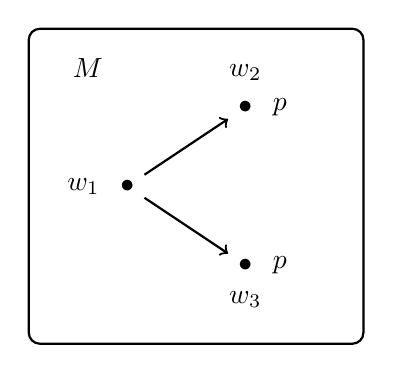
\begin{tikzpicture}[node distance=2cm, auto, thick]
      \node (w1) at (0, 1) [label=180:$w_1$]{$\bullet$}; 
      \node (w2) at (1.5, 2) [label=90:$w_2$, label=right:{$p$}]{$\bullet$}; 
      \node (w3) at (1.5, 0) [label=270:$w_3$, label=right:{$p$}] {$\bullet$};
      \draw[->] (w1) to node {} (w2);
      \draw[->] (w1) to node {} (w3);
      \draw [rounded corners] (-1.25,-1) -- ++(0,4)  -- ++(4.25,0) -- ++(0,-4) --  cycle;
      \path node at (-0.5,2.5) {$\mModel{M}$};
    \end{tikzpicture}
  \end{center}
\caption{Counterexample to $p \lif \Diamond p
  \Entails \Box p \lif p$.}\ollabel{fig:counterex}
  \end{figure}
  
  Often very simple counterexamples suffice. The model $\mModel{M'} =
  \{W', R', V'\}$ with $W' = \{w\}$, $R' = \emptyset$, and $V'(p) =
  \emptyset$ is also a counterexample: Since $\mSat/{M'}{p}[w]$,
  $\mSat{M'}{p \lif \Diamond p}[w]$. As no worlds are accessible
  from~$w$, we have $\mSat{M'}{\Box p}[w]$, and so $\mSat/{M'}{\Box p
    \lif p}[w]$.
\end{ex}

\begin{prob}
  Show that $\Box (!A \land !B) \Entails \Box !A$.
\end{prob}

\begin{prob}
  Show that $\Box (p \lif q) \Entails/ p \lif \Box q$ and $p \lif \Box
  q \Entails/\Box (p \lif q)$.
\end{prob}

\end{document}
